\documentclass[12pt,addpoints,answers]{guia}
\grado{3$^\circ$ de Secundaria}
\cicloescolar{2022-2023}
\materia{Ciencias y Tecnología: Química}
\guia{24}
\unidad{3}
\title{Relaciones entre la estructura y las propiedades de las sustancias}
\aprendizajes{\item Representa y diferencia mediante esquemas, modelos y
              simbología química, elementos y compuestos, así como
              átomos y moléculas.
        \item Explica y predice propiedades físicas de los materiales
              con base en modelos submicroscópicos sobre la
              estructura de átomos, moléculas o iones, y sus
              interacciones electrostáticas.
    }
\author{JC Melchor Pinto}
\begin{document}
\pagestyle{headandfoot}

\INFO
\printanswers
\begin{multicols}{2}
    \include*{../blocks/block000}
\end{multicols}
% \begin{opening}[Atracción electrostática]
%     {Objetivo:\\ Observar el comportamiento de diferentes sustancias ante la presencia de un objeto
%         con carga eléctrica.

%         \begin{minipage}{0.3\textwidth}
%             \begin{figure}
%                 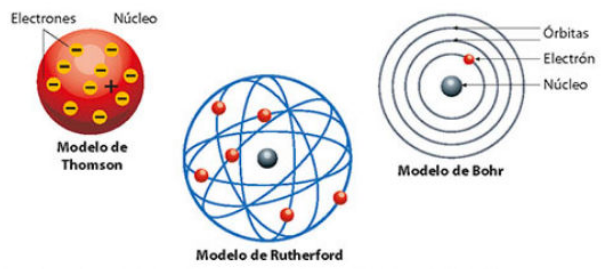
\includegraphics[width=0.9\linewidth]{atomicsmodels}
%                 \caption{Imagen ejemplo del experimento}
%                 \label{fig:}
%             \end{figure}

%         \end{minipage}\hfill
%         \begin{minipage}{0.6\textwidth}
%             Materiales:
%             \begin{itemize}
%                 \item Globo o varilla de plástico o vidrio
%                 \item Franela
%                 \item Bureta o jeringa de 10 mL
%                 \item Vaso de precipitados o de plástico
%                 \item Soporte universal
%                 \item Pinzas de laboratorio
%                 \item Diferentes sustancias líquidas (agua, etanol, acetona, hexano).
%             \end{itemize}

%             Procedimiento:
%             \begin{enumerate}
%                 \item Froten el globo o la varilla de plástico o vidrio con una franela para cargarlo eléctricamente.
%                 \item Predigan, antes de realizar el experimento, si el objeto cargado atraerá, repelerá o no afectará el chorro de cada líquido. Justifiquen sus ideas.
%                 \item Sujeten la bureta al soporte y abran la llave para que salga un chorro de agua delgado, pero continuo.
%                 \item Acerquen el objeto cargado al chorro de agua sin tocarlo. ¿Qué sucede?
%                 \item Repitan el experimento con otros líquidos (etanol, acetona, hexano).
%             \end{enumerate}

%             Análisis de resultados y conclusiones:
%             \begin{enumerate}
%                 \item Contrasten los resultados con sus predicciones.
%                 \item Generen hipótesis iniciales que expliquen por qué los líquidos que utilizaron se comportan de diferente manera.
%             \end{enumerate}
%         \end{minipage}
%     }
% \end{opening}
% \begin{multicols}{2}
% \include*{../blocks/block030a}
% \include*{../blocks/block030b}
% \end{multicols}
\fullwidth{
    \begin{tcolorbox}[enhanced,attach boxed title to top center={yshift=-3mm,yshifttext=-1mm},
            colback=blue!5!white,colframe=blue!75!black,colbacktitle=red!80!black,
            title=Geometría molecular,fonttitle=\bfseries,
            boxed title style={size=small,colframe=red!50!black} ]
        Los materiales que nos rodean están hechos de diferentes sustancias, y sus propie-
        dades dependen de su composición y de la estructura de las partículas que los
        componen. Como hemos visto, las moléculas que conforman las sustancias están
        compuestas por distintos tipos de átomos enlazados de diversas maneras, lo cual
        determina si el material que forman será o no soluble en agua, si a temperatura
        ambiente existirá como líquido o sólido o si lo atraerá o no un cuerpo cargado.
        El tipo de átomos que se combinan para formar una molécula y la manera en la
        que se enlazan determina la \emph{geometría} de la partícula, es decir, la forma que ad-
        quiere; por ejemplo, las moléculas de dióxido de carbono (CO$_2$ ) están compuestas por
        un átomo de carbono unido mediante enlaces dobles a dos átomos de oxígeno organiza-
        dos en una línea. Se dice entonces que la molécula tiene geometría lineal (figura 2.38).
        No todas las moléculas compuestas por tres átomos son lineales. Las moléculas
        de agua H 2 O, por ejemplo, poseen una geometría plana angular debido a repulsiones
        entre los electrones de valencia en el átomo de oxígeno central y en los átomos de
        hidrógeno que lo rodean (figura 2.39).
        \begin{figure}[H]
            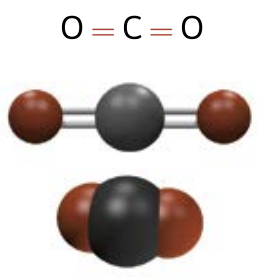
\includegraphics[width=0.45\textwidth]{20230321060221}
            \caption{Diferentes
                representaciones de
                la geometría lineal
                de la molécula de
                dióxido de carbono
                (CO$_2$ ) .}
            \label{fig:20230321060221}
        \end{figure}
        \begin{figure}[H]
            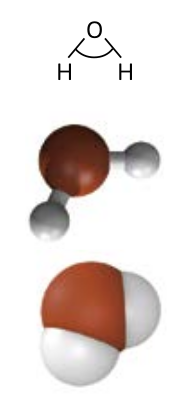
\includegraphics[width=0.45\textwidth]{20230321060418}
            \caption{Distintas
                representaciones
                de la geometría
                plana de la molécula
                de H 2 O.}
            \label{fig:20230321060418}
        \end{figure}
    \end{tcolorbox}
}

\begin{questions}
    hola
    \begin{parts}
        \part adiios
    \end{parts}

    \fullwidth{
        \begin{tcolorbox}[enhanced,attach boxed title to top center={yshift=-3mm,yshifttext=-1mm},
                colback=blue!5!white,colframe=blue!75!black,colbacktitle=red!80!black,
                title=Distribución de carga,fonttitle=\bfseries,
                boxed title style={size=small,colframe=red!50!black} ]
            La composición y geometría de las moléculas determina la forma en que los electro-
            nes de valencia se distribuyen entre los átomos que las conforman, lo cual, a su vez,
            afecta la interacción con otras moléculas. No todos los átomos atraen con la misma
            fuerza a los electrones de valencia que los enlazan. Algunos átomos, como los del flúor
            (F) y el oxígeno (O), atraen a los electrones con más fuerza que los átomos de carbono
            (C) e hidrógeno (H). Cuando un átomo de cloro se enlaza con uno de hidrógeno y ori-
            ginan una molécula de HCl (cloruro de hidrógeno), los electrones que forman el enlace
            pasan más tiempo cerca del átomo de cloro porque los atrae con más fuerza. Esto
            causa que la carga eléctrica no se distribuya uniformemente entre los dos átomos.
            \begin{figure}[H]
                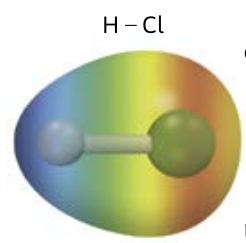
\includegraphics[width=0.45\textwidth]{20230321060047}
                \caption{En la
                    molécula de HCl, la
                    carga electrónica
                    no se distribuye
                    uniformemente entre
                    los dos átomos.}
                \label{fig:20230321060047}
            \end{figure}
            Dado que los electrones tienen carga eléctrica negativa y pasan más tiempo cerca
            del átomo de cloro en la molécula de HCl, la región donde se ubica el átomo de
            cloro es parcialmente negativa mientras la región que rodea al átomo de hidró-
            geno es parcialmente positiva. La molécula es eléctricamente neutra (posee el
            mismo número de protones que de electrones), pero la distribución de electrones
            no es la misma en todas partes. Por lo común, este fenómeno se representa asig-
            nando coloraciones distintas a las regiones negativas y positivas en una molécula.
            Como ilustra la figura 2.40, las zonas parcialmente negativas se colorean con tonos
            más rojizos, mientras las zonas parcialmente positivas con tonos más azulados.
        \end{tcolorbox}
    }
    \fullwidth{
        \begin{tcolorbox}[enhanced,attach boxed title to top center={yshift=-3mm,yshifttext=-1mm},
                colback=blue!5!white,colframe=blue!75!black,colbacktitle=red!80!black,
                title=Electronegatividad,fonttitle=\bfseries,
                boxed title style={size=small,colframe=red!50!black} ]
            El químico Linus Pauling propuso una manera de medir la fuerza con la que diferentes
            átomos atraen a los electrones en un enlace, propiedad que llamó electronegatividad.
            Para los elementos en la
            tabla periódica, la electronegatividad se incrementa
            de abajo hacia arriba y de izquierda a derecha, como
            muestra la figura 2.41.
            Los átomos de los elementos no metálicos poseen una electronegatividad más
            alta que los átomos de los elementos metálicos, lo cual quiere decir que atraen a los electrones en un enlace con
            más fuerza. Dentro de los elementos no metálicos, los átomos de flúor (F) y de oxígeno
            (O) son los más electronegativos mientras que los átomos de hidrógeno (H) y fósforo
            (P) son los menos electronegativos. El análisis de la electronegatividad de los dife-
            rentes átomos que se enlazan en una molécula permite predecir qué regiones de la
            partícula serán parcialmente negativas o positivas. En cualquier enlace químico entre
            dos átomos distintos, el átomo más electronegativo será parcialmente negativo y el
            átomo menos electronegativo será parcialmente positivo.
        \end{tcolorbox}
    }
    \fullwidth{
        \begin{tcolorbox}[enhanced,attach boxed title to top center={yshift=-3mm,yshifttext=-1mm},
                colback=blue!5!white,colframe=blue!75!black,colbacktitle=red!80!black,
                title=Polaridad molecular,fonttitle=\bfseries,
                boxed title style={size=small,colframe=red!50!black} ]
            El análisis de cómo los electrones de valencia se distribuyen entre los áto-
            mos de las moléculas permite clasificarlas en dos grandes grupos. En algu-
            nas moléculas la carga eléctrica se distribuye de manera uniforme entre los
            átomos. Este tipo de moléculas se denominan \emph{no polares}, y las moléculas
            en las que la carga eléctrica no está distribuida de manera uniforme se co-
            nocen como moléculas \emph{polares}. En la figura 2.42 se presentan dos ejemplos
            típicos de estos tipos de moléculas. Esta clasificación es importante porque
            las moléculas polares y las no polares interaccionan de manera distinta en-
            tre ellas y con otras moléculas, lo que les da propiedades distintas a las
            sustancias que se forman con estas partículas.
            \begin{figure}[H]
                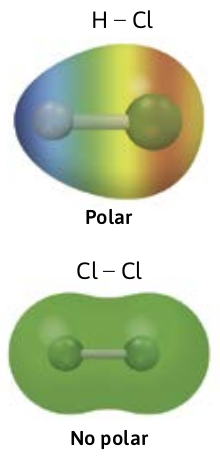
\includegraphics[width=0.45\textwidth]{../images/20230321055533}
                \caption{La molécula de Cl$_2$ es no polar y la de HCl, polar.}
                \label{fig:20230321055533}
            \end{figure}
            \begin{figure}[H]
                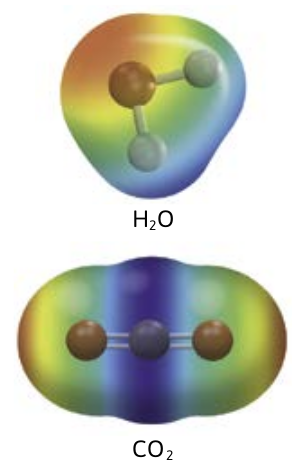
\includegraphics[width=0.45\textwidth]{../images/20230321055646}
                \caption{LLa molécula de H$_2$O es polar pero la de CO$_2$ es no polar.}
                \label{fig:20230321055646}
            \end{figure}
            La polaridad de una molécula (esto es, si es polar o no polar) depende
            de los átomos que la constituyen, de cómo se enlazan entre sí y de la geo-
            metría de la molécula. Cuando las moléculas están formadas sólo por dos
            átomos, la decisión de si son o no polares es más o menos sencilla. Si los áto-
            mos tienen la misma electronegatividad, la molécula no será polar, pero si
            su electronegatividad es distinta, la molécula es polar porque los electrones
            no se distribuyen de manera uniforme entre los dos átomos.
            Si las moléculas tienen más de dos átomos, saber si son o no polares re-
            quiere mayor análisis de la forma en que se distribuye la carga electrónica
            sobre toda la molécula. Considera, por ejemplo, la distribución de la carga
            en las moléculas de CO 2 y H 2 O que se ilustran en la figura 2.43. La molécula
            de H 2 O se considera polar porque en un extremo es parcialmente negativa
            (donde se localiza el átomo de oxígeno) y el lado opuesto (donde están los
            hidrógenos) es parcialmente positivo. Esto es diferente de lo que observamos
            en la molécula de CO 2 , cuya región central, donde se localiza el átomo de
            carbono, es más positiva que las regiones laterales, donde se ubican los áto-
            mos de oxígeno. La distribución de carga en la molécula no es la misma, pero
            ningún extremo de la molécula es más positivo o negativo que el otro; cuan-
            do esto sucede, la molécula es no polar.
        \end{tcolorbox}
    }
    \fullwidth{
        \begin{tcolorbox}[enhanced,attach boxed title to top center={yshift=-3mm,yshifttext=-1mm},
                colback=blue!5!white,colframe=blue!75!black,colbacktitle=red!80!black,
                title=Fuerzas intermoleculares,fonttitle=\bfseries,
                boxed title style={size=small,colframe=red!50!black} ]
            %\centering Conjunto de fuerzas que determinan la interacción entre moléculas.
            Fuerza intermolecular se refiere a las interacciones que existen entre las moléculas conforme a su naturaleza. Generalmente, la clasificación es hecha de acuerdo a la polaridad de las moléculas que están interaccionando, o sobre la base de la naturaleza de las moléculas, de los elementos que la conforman.\\
            Las moléculas que conforman las sustancias están compuestas
            por protones y electrones con carga eléctrica. Por tanto, cuando
            una molécula se acerca a otra, los electrones de una de estas par-
            tículas pueden ser atraídos por los protones de la otra molécula,
            y viceversa; esto causa interacciones atractivas entre las moléculas
            a las que se denomina fuerzas intermoleculares. Estas interaccio-
            nes atractivas con frecuencia se representan con líneas delgadas
            punteadas entre moléculas, como ilustra la figura 2.44.
            Las fuerzas intermoleculares son responsables de que en ma-
            teriales sólidos y líquidos las moléculas se mantengan juntas.
            \begin{figure}[H]
                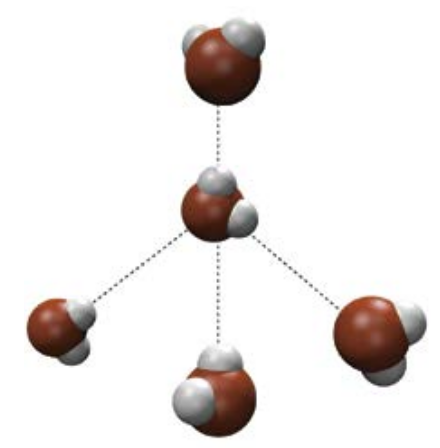
\includegraphics[width=0.45\textwidth]{../images/20230321054752.png}
                \caption{m}
                \label{fig:20230321054752}
            \end{figure}
            Debido a su presencia se debe proporcionar energía para separar
            las moléculas y transformar las sustancias de sólido a líquido o de
            líquido a gas. Con datos experimentales es posible inferir en qué
            sustancias las fuerzas intermoleculares son menores o mayores.
        \end{tcolorbox}
    }
    \fullwidth{
        \begin{tcolorbox}[enhanced,fit to height=5cm,
                colback=green!25!black!10!white,colframe=green!75!black,title=Fit box (5cm),
                drop fuzzy shadow,watermark color=white,watermark text=Fit]
            %\lipsum[1-4]
        \end{tcolorbox}
    }
    % \include*{../questions/question067a}
    % \include*{../questions/question068a}
\end{questions}
\end{document}
